\chapter{EVALUATION}

In this section, we will evaluate the performance of the key components of the system, Information Extraction and the Ontology Similarity respectively, and then the whole system.

\section{Experiments of Information Extraction }

To evaluate the performance of information extraction, we get some sentences by the sentence filters, different sentence filter can extract different kinds of sentences. We use the sentences that have degree information to explain the process:

In the experiment, we selected 100 sentences from job descriptions that are requirements of candidates degree and major. The values of degree and major are labeled manually. We use patterns to  match and extract the degree information from the sentences. The patterns are gotten from the observation of sentences. The Figure~\ref{fig:degree_accuracy} shows that when the number of  patterns increases, the accuracy of information increases as well. When we used 6 patterns, the accuracy of degree became 94\%. The accuracies of three fields matching are shown in Table \ref{tab:ieaccura}

\begin{figure}[htbp]
  \centering
  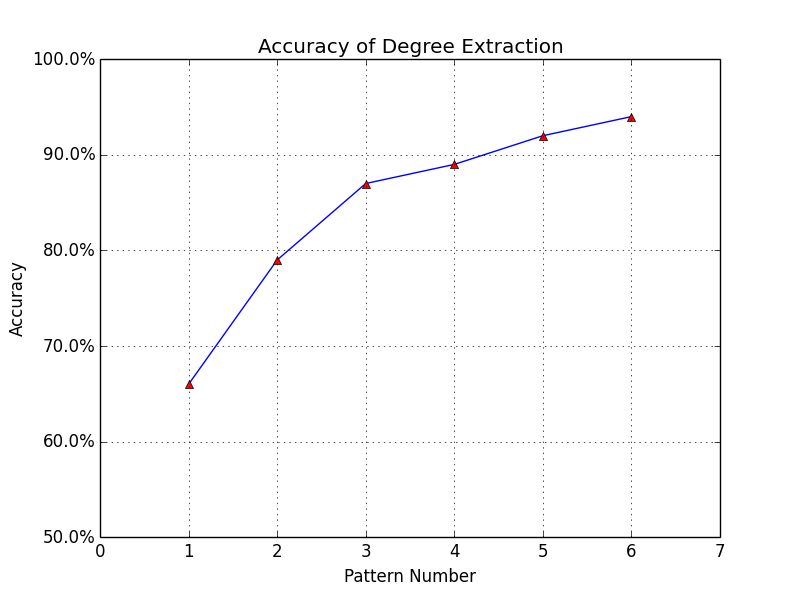
\includegraphics[scale=0.5]{images/degree_accuracy.png}
  \caption{Degree Extraction  Accuracy}
  \label{fig:degree_accuracy}
\end{figure}


\begin{table}[ht]
\caption{Information Extraction} % title of Table
\centering % used for centering table
\begin{tabular}{   | c | c | c | c |   }
 \hline
                     Field   & Pattern Num & Accuracy     \\
 \hline
                     Degree & 6         & 0.94         \\
 \hline
                     Major  & 10        & 0.85      \\
 \hline
                     Skill  & 6         & 0.82      \\
 \hline
\end{tabular}
\label{tab:ieaccura} % is used to refer this table in the text
\end{table}

\section{Experiments of Ontology Similarity}

We select some very common skills from 500 job descriptions, table~\ref{tab:dismatrix3} shows similarity values between these skills. The values in the table are the similarities between skills, the higher the value, the greater of the similarity, so the similarity between one skill and itself is 1. We select one concept, rank other concepts by their similarity value to this concept. The ranked concepts are also be given relevance scores by human judges, so we can use NDCG to evaluate the effectiveness of our approach.

\begin{table}

\caption{Skills Similarity Table 1}
\begin{tabular}{ c | c c c c c c   }
 \hline
  Term       &  Java  &  JDBC  & Spring & Hibernate & MySql  & Oracle   \\  \hline
  Java   &   1    & 0.0523 & 0.091  &   0.0458  & 0.0339 & 0.0608    \\  \hline
    JDBC   & 0.0523 &   1    & 0.0525 &   0.0799  & 0.006  & 0.0616   \\  \hline
   Spring  & 0.091  & 0.0525 &   1    &   0.2008  & 0.0194 & 0.0878   \\  \hline
 Hibernate & 0.0458 & 0.0799 & 0.2008 &     1     & 0.0073 & 0.115    \\  \hline
   MySql   & 0.0339 & 0.006  & 0.0194 &   0.0073  &   1    & 0.049    \\  \hline
   Oracle  & 0.0608 & 0.0616 & 0.0878 &   0.115   & 0.049  &   1      \\  \hline
 \hline
\end{tabular}
\label{tab:dismatrix3}
\end{table}

We use $ Normalized~Discounted~Cumulative~Gain ( NDCG )$ to evaluate the statistical-based similarity. NDCG is an important measure to evaluate the ranked retrieval results. For a set of queries $Q$, let $R(j,d)$ be the relevance score assessors gave to document $d$ for query $j$.
       $$ NDCG(Q,k) = \frac {1}{|Q|} \sum_{j=1}^{|Q|}{Z_{kj}} \sum_{m=1}^{k} \frac{2^{R(j,m)} - 1}{ \log_2(1+m)} $$

Where $Z_{kj}$ is a normalization factor calculated to make it so that a perfect ranking's NDCG at $k$ for query $j$ is 1. For queries for which $k' < k$ documents are retrieved, the last summation is done up to $k'$.

The table ~\ref{tab:simcompare1} shows how we evaluate the similarity between the concept ``Javascript'' and some other concepts. The first column is some skill names, the second column is their similarity values to Javascript, the third column is their positions ranked by the similarity values, and the fourth column is relevance value given by the judges. The NDCG value for concept Javascript is 0.94, and in table ~\ref{tab:simcompare2},  NDCG value for concept HTML is 0.97.

\begin{table}
\centering
\caption{ Javascript Similarity Evaluation : NDCG = 0.94 }
\begin{tabular}{ | c | c | c  | c |  }
 \hline
    Term     &  Similarity Value  &  Position   & Relevance     \\  \hline
    jQuery   &  0.1981            &      4      &   8        \\
     HTML    &  0.2087            &      3      &   4         \\
     CSS     &  0.2439            &      2      &   3   \\
     Java    &  0.0665            &      5      &   1   \\
    Python   &  0.0189            &      8      &   1   \\
     Ruby    &  0.023             &      7      &   1    \\
     JSP     &  0.0253            &      6      &   2    \\
 \hline
\end{tabular}
\label{tab:simcompare1}
\end{table}


\begin{table}
\centering
\caption{ HTML Similarity Evaluation : NDCG = 0.97 }
\begin{tabular}{ | c | c | c  | c |  }
 \hline
    Term      &  Similarity Value  &  Position   & Relevance     \\  \hline
  Javascript   &  0.2087           &      2      &   3        \\
     jQuery    &  0.0979           &      3      &   3         \\
     CSS     &  0.3569             &      1      &   5   \\
     Java    &  0.0473             &      4      &   1   \\
    Python   &  0.0175             &      6      &   1   \\
     Ruby    &  0.023              &      5      &   1    \\
     JSP     &  0.0103             &      7      &   3    \\
 \hline
\end{tabular}
\label{tab:simcompare2}
\end{table}


\section{Evaluation of the System}

In traditional information retrieval system, precision and NDCG are widely used measures ~\cite{manning2008introduction}. Precision ($P$) is the fraction of retrieved documents that are relevant .
       $$  Precision =  \frac{ \#(releveant~items~ retrieved)}{ \#(retrieved~items)}$$

We first used Precision@K to compare the performance our approach to some classical information retrieval models, that are Okapi BM25~\cite{robertson2009probabilistic}, Kullback-Leibler divergence, and the TF-IDF. Precision@K is the proportion of relevant documents in the first K positions and is given below:
$$ P@k = \frac{1}{k} \sum^m_{i=1} l_i 1 \left(  r(i) \leq k  \right )  $$
Where 1 is the indicator function: $1(A) = 1$ if A is true, 0 otherwise.

In the evaluation phrase, we created a data set of 100 job descriptions, which includes several kinds of jobs, like web developers, back-end developers, mobile developers and so on. We used 5 candidate resumes and retrieved the top 20 jobs.  The relevance value of job descriptions to each resume will be set manually. We create a query q from the resume, and treat the text of the job descriptions as documents d and apply standard ad-hoc retrieval techniques to rank the jobs. For our experiments to compare the various retrieval methods, Okapi BM25 ,  Kullback-Leibler divergence, and the TF-IDF. We would like to return jobs that better match the candidates' resumes at the top. The result of Precision@k is in table~\ref{tab:job_precision}.

\begin{table}[ht]
\caption{Precision of Job Ranking } % title of Table
\centering % used for centering table
\begin{tabular}{    | c | c | c | c | c |  }
 \hline
       k     & Okapi BM25 & KL    & TF-IDF   & Ontology Similarity  \\
 \hline
       5     & 0.13       & 0.40  & 0.54     & 0.74   \\
 \hline
       10    & 0.16       & 0.36  & 0.50     & 0.66   \\
 \hline
       20    & 0.16       & 0.35  & 0.49     & 0.61   \\
 \hline

\end{tabular}
\label{tab:job_precision} % is used to refer this table in the text
\end{table}

The other measure we used is NDCG, which is explained in last section. Table ~\ref{tab:job_ndcg} shows the NDCGvalue get from different information retrieval model. The result shows that Ontology Similarity  performs the best. This agrees with results in  where it was found that finding and weighting up important concepts in long queries can improve retrieval performance.

\begin{table}[ht]
\caption{NDCG of Job Ranking } % title of Table
\centering % used for centering table
\begin{tabular}{    | c | c | c | c | c |  }
 \hline
       k    & Okapi BM25 & KL    & TF-IDF & Ontology Similarity  \\
 \hline
       5    & 0.15       & 0.34  & 0.45     & 0.78   \\
 \hline
       10   & 0.18       & 0.44  & 0.47     & 0.72   \\
 \hline
       20   & 0.19       & 0.35  & 0.45     & 0.66   \\
 \hline

\end{tabular}
\label{tab:job_ndcg} % is used to refer this table in the text
\end{table}

\section{User Study}

We evaluated the system by user studies. The purpose of the evaluation is to test the hypothesis that resume-job matching approach could return better results than keywords searching approach.

\subsection{Procedure of User Study}

At the start of the study, the experimenter introduced the system to the users. He introduced the features of the system, and gave a demo of how to the three different methods in the system to search the jobs. Then a subject was given a resume, all the resumes were download from the internet randomly. The user spent approximately 10 minutes to familiar with it, and got initial idea of what jobs are appropriate to the resume. The subject was asked to search a specific kind of job, like web developer or software engineer with the three methods. During the searching process, the time they used to search and the number of jobs they had reviewed for each method were recorded.  At the end of the study, the subject was asked to take a survey that asked  the personal judgment about the results accuracy of the three methods.


\subsection{Results}


Ten users participated user study, they are graduate and undergraduate students of Computer Science department of Texas A\&M University. The basic requirement of the users is that they can understand the meanings of technical terms of job description. The results of the study are shown in Table~\ref{tab:methodcompare}.


\begin{table}[ht]
\caption{Comparatione of Three Searching Methods } % title of Table
\centering % used for centering
\begin{tabular}{  | c | c | c | c | }
 \hline
 Method                    &  Time Used(Minutes)    & Job Reviewed & Accuracy Score  \\
 \hline
 Keyword                   & 6.3                    & 15.8         &       3.2         \\
 \hline
 Resume Matching           & 5.2                    & 14.6         &       4.1         \\
  \hline
 Keyword + Resume Matching & 4.3                    & 13.2         &       4.1       \\
  \hline
\end{tabular}
\label{tab:methodcompare} % is used to refer this table in the text\section{Pipeline of Information Extraction}
\end{table}


